\section{Evaluation}
\label{s:evaluation}


We evaluate the performance of our classifier using F1 scores (see Table~\ref{t:F1_scores}).
In summary, our classifier performs best on Hopper, which yields an F1 score of 0.88 (with the RBF kernel).
Our classifier performs worst on Sandy, on which it achieves an F1 score of 0.75 (also using the RBF kernel).
On all three machines, the RBF kernel outperforms the MLP kernel.

\begin{table}[t]
    \begin{center}
        \begin{tabular}{c|c|c}
            Machine & RBF Kernel & MLP Kernel \\ \hline
            Emerald & 0.82 & 0.64 \\
            Hopper & 0.88 & 0.82 \\
            Sandy & 0.75 & 0.59 \\
        \end{tabular}
    \end{center}
    \caption{F1 scores for each machine and kernel. Note that on all machines, the RBF kernel outperformed the MLP kernel.}
    \label{t:F1_scores}
\end{table}

In order to measure how many datapoints are required to train an accurate classifier, we explored the effects of reducing the size of our training set.
In this experiment, we randomly selected X\% of our original 1000 training points, for X ranging from 1\% to 100\%.
After training our classifier with this random X\% of training data, we measured the resulting F1 score on the test data. See Figure~\ref{fig:convergence}.

\begin{figure*}[t]
    \centering
        \begin{subfigure}[t]{0.33\textwidth}
            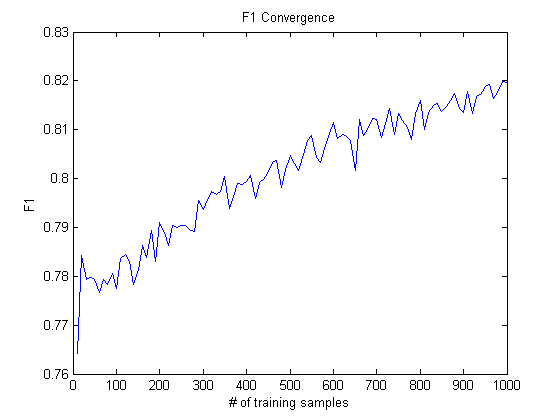
\includegraphics[width=\textwidth]{figures/F1_convergence_emerald.png}
            \caption{Emerald}
            \label{f:F1_emerald}
            \end{subfigure}
        \begin{subfigure}[t]{0.33\textwidth}
            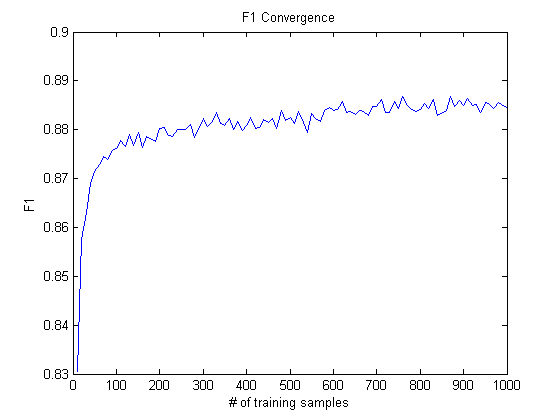
\includegraphics[width=\textwidth]{figures/F1_convergence_hopper.png}
            \caption{Hopper}
            \label{f:F1_hopper}
        \end{subfigure}
        \begin{subfigure}[t]{0.33\textwidth}
            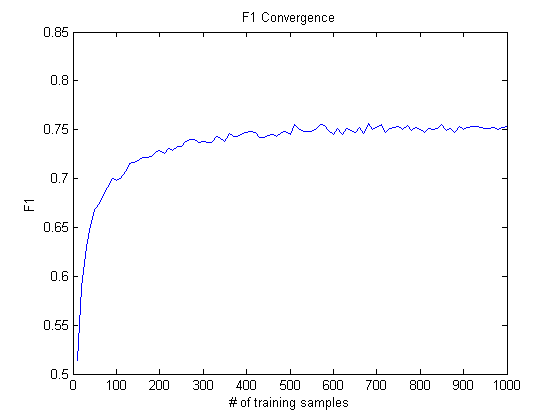
\includegraphics[width=\textwidth]{figures/F1_convergence_sandy.png}
            \caption{Sandy}
            \label{f:F1_sandy}
        \end{subfigure}
        \caption{F1 convergence on each machine (using the RBF kernel). Sandy and Hopper require fewer than 500 datapoints to generate accurate performance models, while Emerald requires more than 1000 (due to Emerald's more complicated performance patterns).}
    \label{fig:convergence}
\end{figure*}

Of course, the number of training points required to build an accurate model will vary widely by machine and algorithm.
As shown in Figure~\ref{fig:convergence}, although Sandy and Hopper require fewer than 500 datapoints to achieve a maximal F1 score, Emerald requires more than 1000.
This is due to the fact that performance patterns on Emerald are more complex.
We don't have a theoretical model to understand this complexity, further validating the value our empirical approach.

We also performed tests to quantify the benefit of using our algorithm selection technique.
How much do we gain by using our classifier to select the optimal algorithm?
It depends on the machine, as well as what algorithm would have been chosen otherwise.
For example, using our classifier on Emerald yields an 11.3\% average speedup over using only CARMA, and a 5.7\% speedup over using just MKL (this includes the penalties of misclassifications).
On Hopper, our classifier enjoys a healthy 28.0\% gain over using MKL only.
For complete results, see Table~\ref{t:improvements}.

\begin{table}[t]
    \begin{center}
        \begin{tabular}{c|c|c}
            Machine & Selection vs CARMA Only & Selection vs MKL Only \\ \hline
            Emerald & 11.3\% & 5.7\% \\
            Hopper & 2.2\% & 28.0\% \\
            Sandy & 4.4\% & 0.9\% \\
        \end{tabular}
    \end{center}
    \caption{F1 scores for each machine and kernel. Note that on all machines, the RBF kernel outperformed the MLP kernel.}
    \label{t:improvements}
\end{table}
